
\documentclass[12pt]{article}
%\usepackage[left=3.5cm, right=3.5cm]{geometry} % margins for title page. changed below.

\usepackage{hyperref}
\usepackage{fancyvrb} 
\DefineShortVerb{\|} % verbatim code formatting. example: |void foo();|
\usepackage{setspace} % spacing

\title{Better Query Completion}

\author{
Andreas Cederholm (ance@kth.se)
\and
Victor Hung (vhung@kth.se)
\and
Christopher Norman (chnor@kth.se)
\and
Jonathan Pellby (jonathp@kth.se)
\and
Martin Runelöv (mrunelov@kth.se)
}
\date{\today}

\begin{document}
\maketitle
\thispagestyle{empty}
%\pagebreak
\thispagestyle{empty}
\mbox{}
%\newpage
\setcounter{page}{1}

%\newgeometry{right=2.5cm,left=2.5cm} % Set LR margins for the rest of the document

\begin{abstract}
This project looks at new ways to utilize query completion for advanced users of Apache Solr, with knowledge of the underlying structure of the data. The main goal is to enable query completion for field names, and data within specific fields when a field is present within the query. This has been done by implementing a custom Suggester component for Apache Solr. With the help of this component advanced users can more quickly find what they are looking for, with total recall and maximal precision.
\end{abstract}

\pagebreak
\thispagestyle{empty}
\mbox{}
%\newpage

\doublespacing % more spacing in TOC
\tableofcontents
\singlespacing % turn off double spacing
\pagebreak

\section{Introduction}\label{introduction}
Query completion, or autocomplete, is a feature commonly seen in web browsers, email clients, source code editors and other programs that provides search capabilities to the user. The core principle in query completion is to predict what the user is typing and give suggestions based on that prediction. If the prediction is correct it will speed up typing and may also help the user find the words to express what he or she is searching for. 

Apache Solr is the most popular enterprise search engine as of April 2014\cite{RANKINGS} and is used by many prominent services such as Netflix, The Guardian, AOL and Instagram \cite{SOLR::USAGE}. It supports many advanced features for searching, among which query completion is one. A central part of Solr is the concept of fields. A field can be for example a name, category or price. Documents are organized based on such fields and it is possible to do field queries to find all documents where a field is set to a specific value. For a more advanced user, this is a key concept that greatly enhances the users capabilities of finding the right documents, especially when the search domain is known. 

Despite fields being such a powerful tool when searching, the query completion in Apache Solr is limited to free text queries. It is therefore of great interest to create a module for query completion of field queries. Doing so could not only increase effectiveness for advanced users, but also introduce less experienced users to using fields in their searches.


\subsection{Problem domain}

The aim of this project is to implement a module for Apache Solr that complements the current query completion in Solr so that it supports field querying. The goal is that the user should be able to get query completion for field names in the following manner:
\begin{enumerate}
\item   If the user types |aut|, and there is a field called author in the schema, the module will suggest |author:”|. 
\item   If the user types |author:”Joan|, and there is a document authored by Joanne Kathleen Rowling, the module will suggest |author:”Joanne| and |author:”Joanne Kathleen Rowling|
\end{enumerate}

The results in the examples above may vary depending on how the Solr server is configured. For example, in the second example, only one of the two might be returned, depending on whether the field contents are tokenized or not. 



% \paragraph{Outline}
% The report is organized as follows.
% Section~\ref{conclusions} gives the conclusions\cite{Gil:02}.


\section{Background}\label{background}

The original purpose of query completion was to help people with physical disabilities improve their typing speed (Tam, C. \& Wells, D. (2009). Evaluating the Benefits of Displaying Word Prediction Lists on a Personal Digital Assistant at the Keyboard Level. Assistive Technology, 21, 105-114.). It later evolved to incorporate a lot more and today it is seen almost everywhere on both the Internet and in software tools and applications. Popular search engines such as Google and Microsoft Bing (https://www.google.se/ , www.bing.com ) as well as popular text editors and IDEs such as Sublime Text and Eclipse has query completion implemented (https://www.eclipse.org/ , http://www.sublimetext.com/).

\subsection{Previous work}\label{previouswork}

Predicting words is not a trivial thing to do and currently there is extensive research being conducted in this field. This research can vary from implementing an efficient prediction of words to implementing a semantically consistent prediction sequence. Often it is desirable to have an implementation that is both efficient in terms of query processing and response time as well as semantically consistent predictions in order to give the user both fast and correct predictions. This is what most research papers today aims to explore with the emphasis being placed on producing semantically consistent suggestions [Qiaozhu Mei, Dengyong Zhou, and Kenneth Church. 2008. Query suggestion using hitting time. In Proceedings of the 17th ACM conference on Information and knowledge management (CIKM '08). ACM, New York, NY, USA, 469-478] 
[Silviu Cucerzan and Ryen W. White. 2007. Query suggestion based on user landing pages. In Proceedings of the 30th annual international ACM SIGIR conference on Research and development in information retrieval (SIGIR '07). ACM, New York, NY, USA, 875-876]. 

\subsection{Apache Solr}

Apache Solr is an open source free text search platform written in Java. It runs as a standalone search server within a servlet container. It has a REST-like API that supports HTTP requests with e.g. XML and JSON. It is designed to be highly customizable, allowing for easy customization through its configuration files.
[https://lucene.apache.org/solr/]

Consider for instance that we have a document that looks like the following:

\begin{verbatim}
<add>
  <doc>
    <field name="id">SP2514N</field>
    <field name="name">Samsung SpinPoint P120 SP2514N - hard drive - 250 GB</field>
    <field name="manu">Samsung Electronics Co. Ltd.</field>
  </doc>
  ...
</add>
\end{verbatim}

Let us further assume that we store the document on the server and want to retrieve it using solr queries. For instance, we can do this by retrieving all documents containing the word ''samsung'' in the field ''name'', in which case the query would look like:

\begin{verbatim}
http://localhost:8983/solr/collection1/select?q=name:samsung
\end{verbatim}

Which should return the above sample document if it currently indexed in the document set\footnote{Called a core in Solr terminology} |collection1| and the server is currently running on the local host.

A few things to note about the Solr implementation: First, all documents indexed must be flat, i.e. all  field must be immediate children of the |<doc>| tag and the document may not be arbitrarily nested. Second, the returned results is highly dependent on how the server is configured. The above example for instance assumes that the contents of the field “name” is tokenized using whitespace as delimiters and that each resulting token is lowercased. The contents of the field “id” on the other hand may be specified not to use either whitespace tokenization or transforming the tokens to lower case, in which case only the exact query would match the above document:

\begin{verbatim}
http://localhost:8983/solr/collection1/select?q=id:SP2514N
\end{verbatim}

but the following query would not match the above document:

\begin{verbatim}
http://localhost:8983/solr/collection1/select?q=id:sp2514n
\end{verbatim}

Much of the work in setting up a Solr server thus lie in specifying sensible types for the document contents, such that the server allows the user to select the documents they are looking for. In the above for instance it might make sense to distinguish between ''SP2514N'' and ''sp2514n'' as these might refer to different documents, but not to distinguish between ''Samsung'' and ''samsung''.

Solr comes with a built in suggester implementation, for instance performing a query:

\begin{verbatim}
http://localhost:8983/solr/collection1/suggest?sp
\end{verbatim}

will return suggestions consisting of all words beginning with ‘’sp’’ using word from the indexed documents. Which field to use to draw suggestions can be specified by setting a parameter in the configuration file solrconfig.xml. Thus, in principle one can retrieve suggestions from different fields with the current suggester implementation by creating multiple suggesters, one for each field, and querying these independently.








\section{Method}\label{method}

In this section the different components of the project are described. It gives an account of how the query completion module has been implemented. A frontend has also been implemented to provide a better environment for testing and demoing. Lastly, the section contains details on how the implementation was tested and what requirements the implementation should fulfill. 

\subsection{Implementation}

As previously mentioned, Apache Solr has built-in support for free text search. It is contained in the class |org.apache.solr.spelling.suggest.Suggester| and is configured in the file |solrconfig.xml|. In order to implement our query suggestion, a new class, |SuggesterMK2|, has been implemented which piggybacks on the existing functionality of the original Suggester class.\cite{SUGGESTER}

The |SuggesterMK2| implementation attempts to be a drop-in replacement for the Suggester class. Notable exceptions to this general rule include:
\begin{itemize}

\item The |SuggesterMK2| uses the query parameter |spellcheck.q| instead of the parameter |q|
\item The |SuggesterMK2| uses a custom field in |solrconfig.xml| called |delegate| instead of the field called |field|.
\end{itemize}

The rationale for these seemingly arbitrary decisions will be stated explicitly in the coming sections of this report.

\subsubsection{Delegation}

The |SuggesterMK2| implementation uses the delegation pattern\cite{DELEGATE} in order to reuse the original suggester implementation as much as possible. Reusing the original Suggester class means that we can use its query suggestion implementation, as well as its loading and reloading implementations, all of which we can assume work and would be distinctly tricky to implement from scratch.

\begin{figure}[h!]
    \centering
    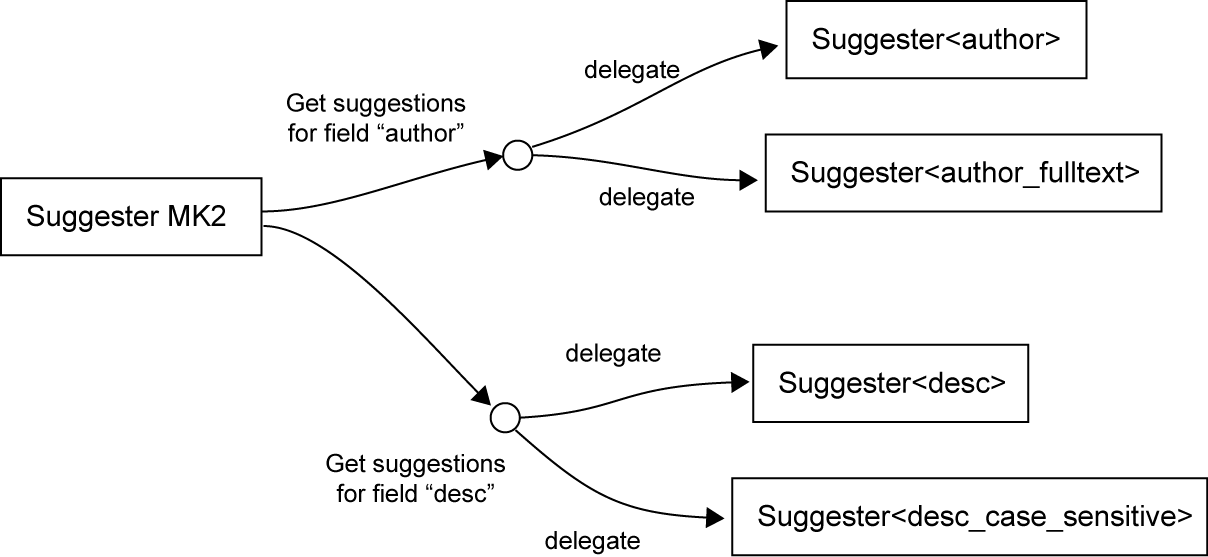
\includegraphics[width=0.8\textwidth]{img/delegation.png}
    \caption{Illustration of the delegation used by SuggesterMK2. The suggester will give suggestions drawn from the fields author and author\_fulltext for the field author, and from desc and desc\_case\_sensitive for the field desc.}
    \label{fig:delegation}
\end{figure}

Let us for instance say that we configure the system to give suggestions for the field |author| using the contents from the fields |author| and |author_exact|, the first of which being tokenized on whitespace, and the second being untokenized. All we have to do then, using delegation, is to construct a |Suggester| object for |author| and |author_exact|, query each of these, and then combine the results, merging results as needed if the results overlap. In our implementation, configuring the suggester to return results as in the diagram can be done by adding the following to the suggester configuration in |solrconfig.xml|:

\begin{verbatim}
<lst name="delegate">
  <str name="targetField">author</str>
  <str name="sourceField">author</str>
  <str name="sourceField">author_fulltext</str>
</lst>
\end{verbatim}

The fields we use for contents do not need to include the target field – we can use the contents from entirely different fields to use as suggestions. For a sample use case where this might be desired, consider what would happen if the target field were 4-gram tokenized: a word like ''parallelize'' would then be split up into the tokens ''para'', ''aral'', ''rall'', ''alle'', and so on, none of which we want to give as query suggestions. We would then want to draw suggestions from some other field where the contents are tokenized as words instead.

The |SuggesterMK2| implementation also gives query suggestions consisting of the field names it is configured to give suggestions for. For instance, the example configuration in figure \ref{fig:delegation} the |SuggesterMK2| would give |author:”| as a query suggestion when the user types |aut|.

For the full configuration of the suggester in solrconfig.xml, see Appendix.
For the implementation of the SuggesterMK2, see \cite{GITHUBPROJ}.

\subsubsection{Order of results}

The results of a query are returned in a given order. Field names are given priority over field contents, while field contents and standard results are both sorted based on number of occurrences. For example of this see section \ref{results}.

\subsubsection{Testing}

A simple frontend has been implemented to act as a tool for debugging and demoing the project. It uses JSON requests and responses to interact with the ''suggest'' and ''select'' features of the Solr server.

Testing was primarily done using the Solr Admin console and the frontend.
In the early stages of development, test data provided by Solr was used. This was replaced with a larger test set of documents containing fields for names, party affiliation and quotes from members of Swedish parliament later on. A number of queries were used to test that the suggester performed as expected. These queries, as well as the result of the tests for the final version, can be found in the following section. 


\section{Results}\label{results}

\section{Conclusions}\label{conclusions}
blah blah blah...

\bibliographystyle{abbrv}
\bibliography{references}

\end{document}